

\section{Methods}

% We should probably cite \citet{braun2006using} here...
This study aims to understand the perception of computer science students with regards to climate change and how their field affects and is affected by climate change. To gauge these opinions, we conducted 5 semi-structured interviews with students varying from undergraduate, graduate and doctoral levels. In this section we describe how we collected the data, extracted themes and deduced results from the data.

\subsection{Materials and Procedure}
The semi-structured interview included 13 questions that are tailored to provide insights for our research questions. Q1-Q5 collected demographic information on participant name, gender, age and area of expertise. Q6 was a general warm-up question about the participant’s professional plan for the future. Q7-Q9 were used to answer “How climate change was perceived in daily life?”. Q10-Q11 aimed to find out “How climate change would influence their area of expertise?”. Q12-Q13 discovered “What opportunities were presented in terms of alleviating the effects of climate change?”. 

There were a total of 5 interviews conducted. The interviews were all semi-structured and most questions came from the interview guide that was made explicit above. There were other follow-up questions raised depending on the answers of the interviewee during the interview process. The interviews were conducted online using a video messaging platform called Zoom \footnote{https://zoom.us/} and all of them lasted approximately 20 minutes each. The interviews were recorded with permission and transcribed afterwards. 
\subsection{Analysis}
After conducting the interviews and collecting the data, we analysed it using the following process.

\emph{Generating and collating initial codes}: Each interview was transcribed and bundled into one document. Every author of the paper was given a copy of the final transcript and annotated them individually without communication or interference from other authors, extracting initial codes from the interviews. After being generated, they were collated and collapsed by the similarity of their content, then displayed as sticky notes using a collaborative whiteboard platform called Miro \footnote{https://www.miro.com}. Figure \ref{fig:initial-codes} shows an example of initial codes created by one of the authors.

\begin{figure}
    \centering
    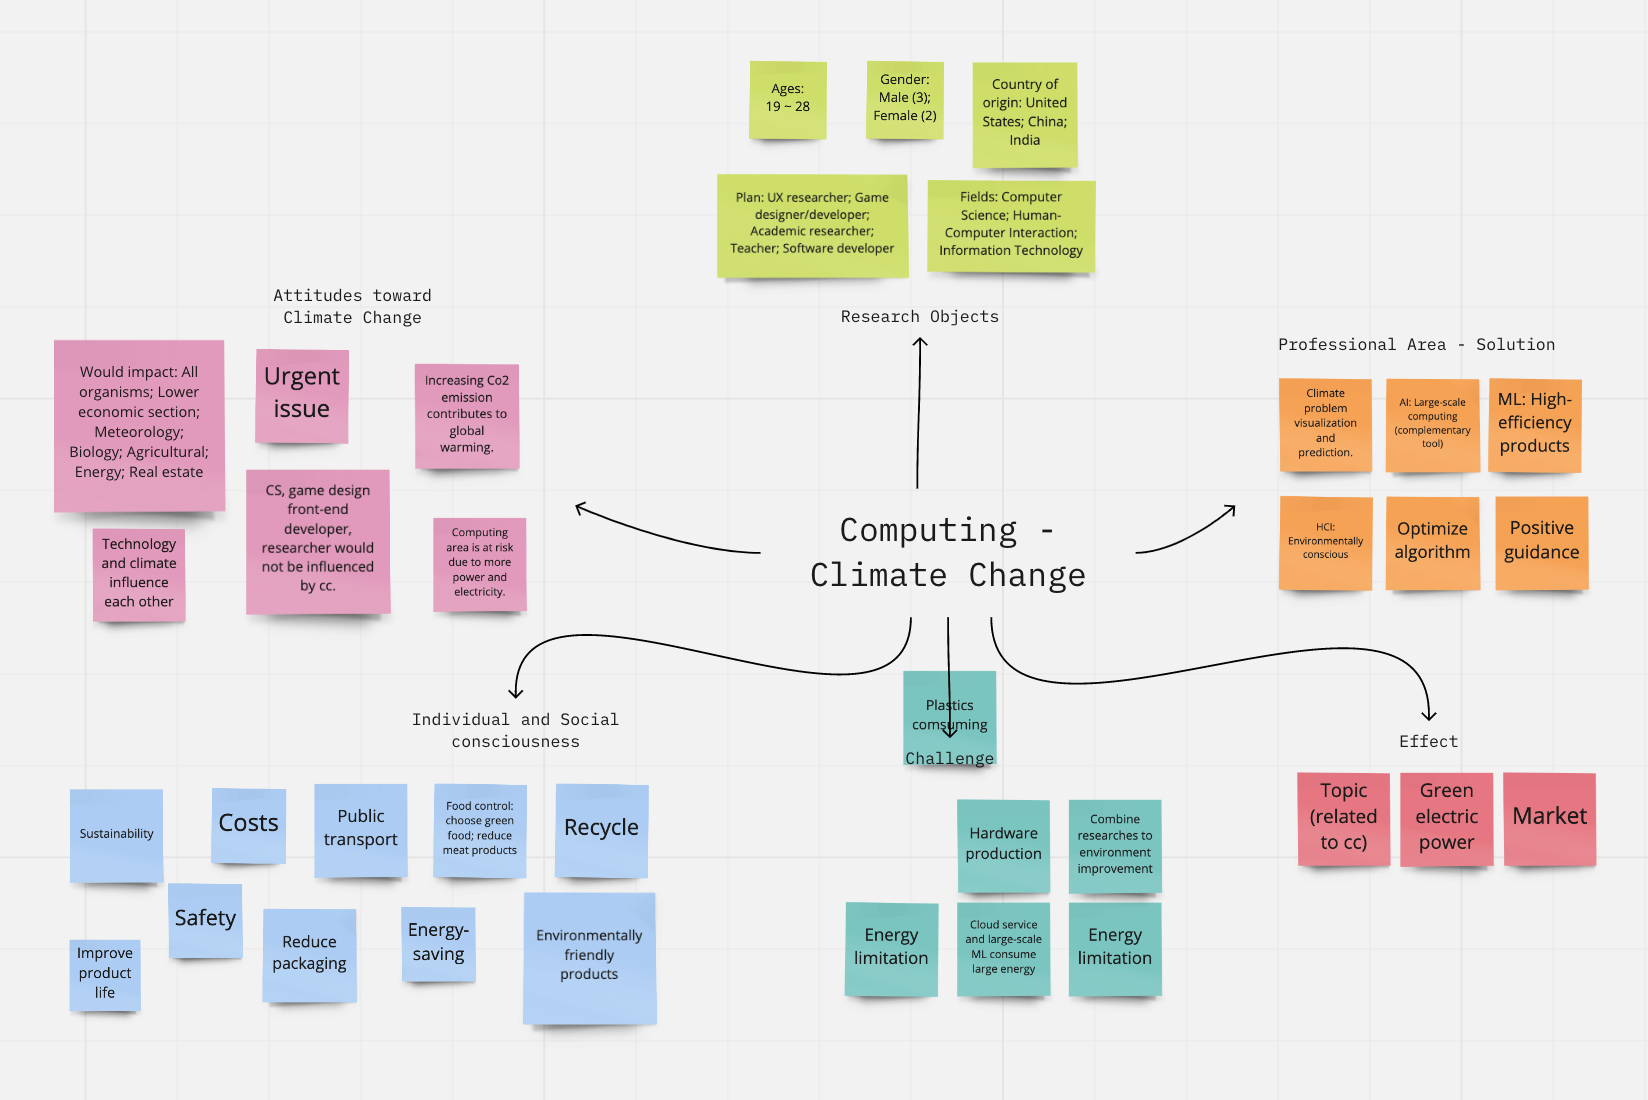
\includegraphics[scale = 0.2]{Figures/Initial Codes.png}
    \caption{Example of Initial Codes}
    \label{fig:initial-codes}
\end{figure}

\emph{Defining themes}: After we put all the initial codes in the same place, the authors grouped together and reviewed our overall coding diagram to identify similarities that allowed thematic grouping. We ended up identifying 4 major categories of themes and attached the codes to the themes if it fits into the category. Figure \ref{fig:theme-codes} illustrates this process. All four themes provide insights to our research questions for the “perception of climate change” and  the “impact on area of expertise”.

\begin{figure}
    \centering
    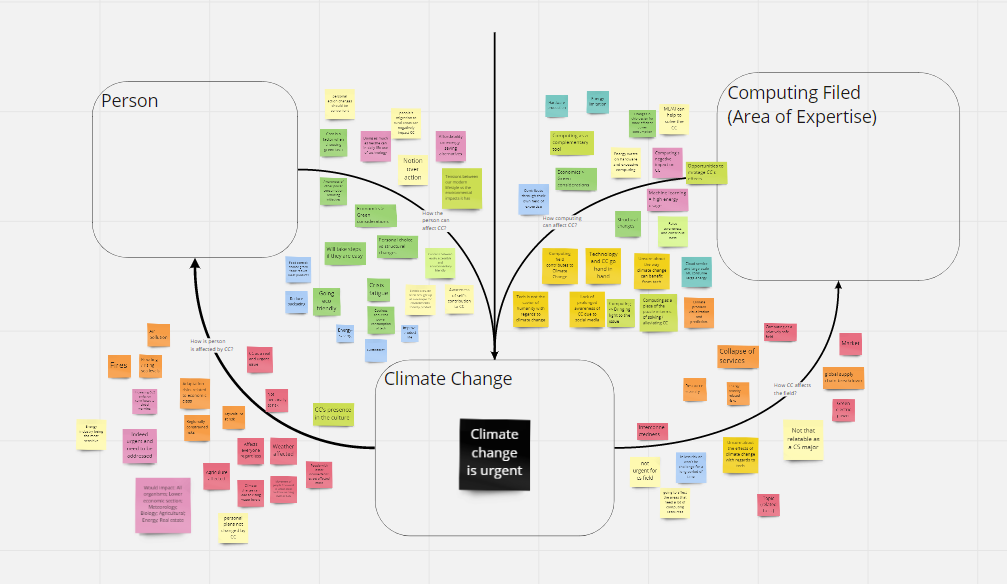
\includegraphics[scale = 0.2]{Figures/codes.png}
    \caption{Themes and their corresponding codes}
    \label{fig:theme-codes}
\end{figure}


